\chapter{Contribution}

Most important chapter of the thesis. Describes what the author contributes as research. Discusses intuition, motivation, describes and reasons about necessity of proposed elements. Defines theses based on reasonable assumptions. Discusses relevant aspects of contribution. Approximately 30 to 40 pages. Can be split into multiple chapters.
\\\\

\section{Baumlayout}

\subsection{Linear vs. Radial}
Aufgrund des begrenzten Platzes, der auf mobilen Geräten typischerweise zur Verfügung steht, war früh in der Entwicklung zu entscheiden, wie Baumstrukturen möglichst platzsparend anzuordnen sind, ohne Übersichtlichkeit einzubüßen. Betrachtet wurden dabei speziell die allgemein übliche Darstellung (linear) gegenüber einer kreisförmigen (radialen) Anordnung.\\
\begin{figure}
	\centering
	\begin{minipage}{.5\textwidth}
		\centering
		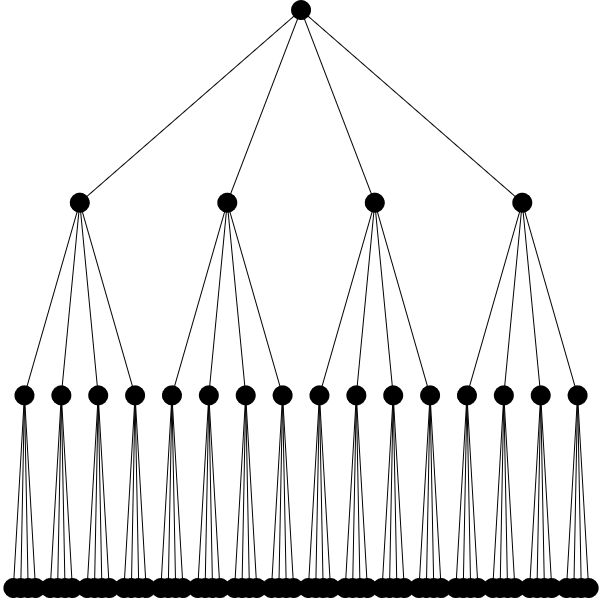
\includegraphics[width=.9\linewidth]{../screenshots/lineargraphexample.PNG}
		\caption{Lineare Baumdarstellung}
		\label{abb:linearbaum}
	\end{minipage}%
	\begin{minipage}{.5\textwidth}
		\centering
		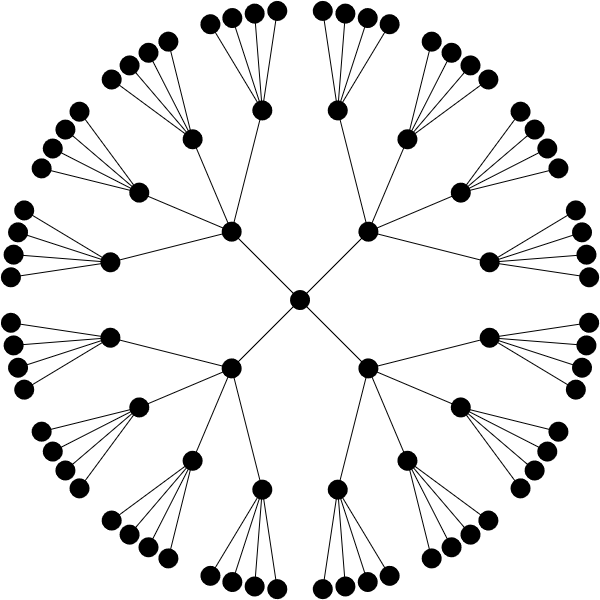
\includegraphics[width=.9\linewidth]{../screenshots/radialgraphexample.PNG}
		\caption{Radiale Baumdarstellung}
		\label{abb:radialbaum}
	\end{minipage}
\end{figure}
Die Abbildungen \ref{abb:linearbaum} und \ref{abb:radialbaum} zeigen einen Vergleich zwischen einem Baum in linearer (Abb. \ref{abb:linearbaum}) und in radialer Anordnung (Abb. \ref{abb:radialbaum}). In beiden Fällen ist derselbe Baum der Höhe 4 auf gleicher Fläche abgebildet. Er besteht aus 105 Knoten, wobei alle inneren Knoten jeweils vier Nachfolger haben. Der Wurzelknoten befindet sich beim linearen Layout am oberen Rand. Die übrigen Knoten sind in drei horizontalen Linien darunter angeordnet, wobei die Kinder der Wurzel auf der obersten Linie liegen, deren Kinder auf der mittleren und deren Kinder auf der untersten Linie. Beim radialen Layout ist die Wurzel in der Mitte abgebildet und alle anderen Knoten in drei konzentrischen Kreisen darum herum. Knoten der Tiefe 1 liegen auf dem innersten Kreis, der Tiefe 2 auf dem mittleren Kreis und die Blätter auf dem äußeren Kreis. Den Mittelpunkt der Kreise bildet die Wurzel. Man sieht deutlich, dass im Fall der vertikalen Anordnung (Abb. \ref{abb:linearbaum}) nicht ausreichend Platz für alle Blätter zur Verfügung steht, wodurch es zu starken Überschneidungen kommt. In der radialen Anordnung (Abb. \ref{abb:radialbaum}) können hingegen alle Knoten überschneidungsfrei dargestellt werden.\\
Um den Grund dafür zu veranschaulichen vergleicht man den Platz, der bei den beiden Herangehensweisen auf einer einzelnen Stufe des Baumes zur Verfügung steht. Unter der Annahme, dass für die gesamte Darstellung ein Quadrat mit Seitenlänge $a$ zur Verfügung steht und alle Knoten einen Durchmesser von 1 haben ergibt sich für den Platz $l_{linear}$ bzw. $l_{radial}$, der auf einer Stufe des Baumes verfügbar ist 
\begin{align*}
&l_{linear} = a\\
&l_{radial} = 2 \cdot \pi \cdot r\mspace{40mu} mit\quad 0\leq r \leq \frac{a}{2} .
\end{align*}
Dabei bezeichnet $r$ den Abstand einer Stufe zum Wurzelknoten. Setzt man $l_{radial}$ und $l_{linear}$ gleich und stellt nach $r$ um, so ergibt sich
\begin{align*}
&l_{linear} = l_{radial}\\
\Rightarrow \mspace{40mu} &a = 2 \cdot \pi \cdot r\\
\Rightarrow \mspace{40mu} &\frac{a}{2 \cdot \pi} = r\\
\Rightarrow \mspace{40mu} &r \approx \frac{a}{6}.
\end{align*}
Da $l_{linear}$ konstant ist kann man daraus ableiten
\begin{align*}
l_{radial} > l_{linear} \mspace{40mu} \Leftrightarrow  \mspace{40mu} r > \frac{a}{6}.
\end{align*}
Das bedeutet, dass ab einem Abstand zur Wurzel von mehr als $\frac{a}{6}$ im radialen Layout mehr Platz für jede Stufe verfügbar ist. Außerdem gilt: Je größer der Abstand $r$, desto mehr Platzersparnis. Das ist vor allem deshalb von Interesse, weil Bäume in der Regel die Eigenschaft haben, dass mit wachsender Baumtiefe auch die Anzahl der Knoten in der jeweiligen Tiefe wächst und diese tiefer liegenden Knoten in der kreisförmigen Darstellung weiter von der Wurzel entfernt sind. Das radiale Layout bietet somit genau dann mehr Platz, wenn üblicherweise mehr Platz benötigt wird.\\
Aufgrund dieser Erkenntnis und der Tatsache, dass beide Darstellungsformen gute Übersichtlichkeit aufweisen, fiel die Wahl letztendlich auf das radiale Layout.

\subsection{Polarkoordinaten}
D3 bietet zur Berechnung einer sinnvollen Knotenanordnung von Bäumen die Funktion $d3.tree()$ an, welche unter Verwendung des Reingold-Tilford Algorithmus \todo{quelle} allen Knoten eines Baumes x- und y-Koordinaten jeweils im Bereich von 0 bis 1 zuordnet. Es liegt dann in der Hand des Programmierers, diese sinnvoll zu interpretieren. Um die Knoten, wie in Abbildung \ref{abb:radialbaum} gezeigt in konzentrischen Kreisen anzuordnen, eignen sich Polarkoordinaten ausgezeichnet. Die y-Koordinate wird als Radius $\rho$, die x-Koordinate als Polarwinkel $\varphi$ in Radiant interpretiert. \todo{bild}
\begin{align*}
&\rho = y\\
&\varphi = 2 \cdot \pi \cdot x
\end{align*}
Zur Darstellung auf dem Bildschirm müssen $\rho$ und $\varphi$ anschließend in kartesische Koordinaten $x_{screen}$ und $y_{screen}$ umgerechnet werden. Die allgemeinen Umrechnungsformeln ergeben sich als
\begin{align*}
&x_{screen} = \rho \cdot \cos (\varphi)\\
&y_{screen} = \rho \cdot \sin (\varphi)
\end{align*}
Bei dieser Umrechnung wird allerdings noch nicht berücksichtigt, dass die gegebenen Polarkoordinaten auf generischen Koordinaten im Bereich $[0,1]$ basieren. Zur korrekten Positionierung müssen noch eine Skalierung auf die verfügbare Breite (width) $w$ und Höhe (height) $h$, sowie eine Verschiebung in die Mitte der Anzeige vorgenommen werden. Es entstehen die endgültigen Formeln:
\begin{align}
&x_{screen} = \rho \cdot \cos (\varphi) \cdot w + \frac{w}{2} \label{eq:polkarthx}\\
&y_{screen} = \rho \cdot \sin (\varphi) \cdot h + \frac{h}{2}.\label{eq:polkarthy}
\end{align}
Nachdem mit dem radialen Layout eine erste Maßnahme zum Einsparen von Platz ergriffen wurde, stellt sich als nächstes die Frage, wie die Übersichtlichkeit weiter verbessert werden kann.


\section{Reduzieren der angezeigten Knoten}

\subsection{Relevante und irrelevante Knoten}
Da Knoten auf dem Bildschirm später Informationen in Form von Text beinhalten sollen, ist es abzusehen, dass jeder einzelne Knoten mehr Platz einnehmen wird, als z.B. in Abbildung \ref{abb:radialbaum} gezeigt ist. Es bietet sich an, immer nur aktuell relevante Knoten ein- und irrelevante auszublenden. Das erfordert je nach Eingabe dynamische Änderungen an der Anzeige der Baumstruktur (Kapitel \ref{sec:dynamische_aktual}). Zunächst muss jedoch entschieden werden, welche Knoten aktuell relevant oder irrelevant sind. 
\begin{figure}
	\centering
	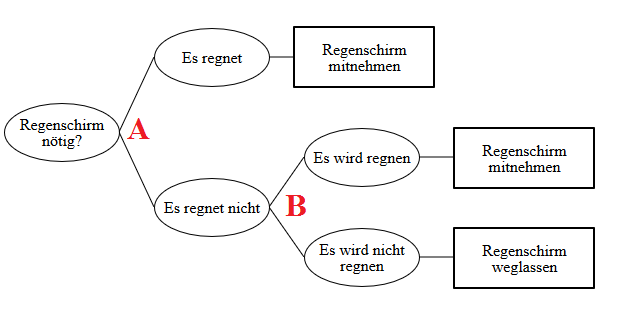
\includegraphics{../screenshots/entscheidungsbaum_bsp.PNG}
	\caption{Ein simpler Entscheidungsbaum}
	\label{abb:entsch_baum_bsp}
\end{figure}
In Abbildung \ref{abb:entsch_baum_bsp} ist beispielhaft ein Entscheidungsbaum zu sehen, der in stark vereinfachter Form die Entscheidungsfindung zur Frage ob ein Regenschirm nötig ist darstellt. Innere Knoten sind als Ellipsen dargestellt und Blätter, welche endgültige Ergebnisse repräsentieren, sind rechteckig. Die Beschriftung der Knoten zeigt an, welche Aussage oder Frage sie symbolisieren. Die beiden Stellen, an denen Entscheidungen getroffen werden müssen, sind mit $A$ und $B$ markiert. In der Situation $A$ gilt es zu entscheiden, ob es regnet oder nicht regnet. Um diese Entscheidung treffen zu können, ist nicht relevant, ob es zu einem späteren Zeitpunkt regnen wird oder nicht und welche Ergebnisse sich daraus ableiten lassen. Bei $B$ wiederum sind vorherige Entscheidungsmöglichkeiten nicht von Interesse, ebenso wie die Folgen davon, ob es regnen wird oder nicht. Man kann sagen, dass bei jeder Verzweigung nur die zur Verfügung stehenden Alternativen relevant sind und angezeigt werden müssen. Da es jedoch nicht nur darum geht, so viel Platz wie möglich zu sparen, sondern auch darum, eine übersichtliche und intuitiv Verständliche Darstellung zu finden ist es hilfreich, außerdem noch den Knoten, von dem die Verzweigung ausgeht zu zeigen. Bei $A$ also den Knoten ``Regenschirm nötig'', bei $B$ ``Es regnet nicht''. Auf diese Art ist es leichter die Orientierung zu behalten, selbst wenn ein Großteil des Baumes nicht sichtbar ist.

\subsection{Dynamische Aktualisierung}\label{sec:dynamische_aktual}

